\section{Experiments linked to the theory}\label{sec:experiments}
\subsection{Design, estimators, and Monte Carlo uncertainty}
The primary design was recorded after the main derivations and before execution. It contains 81 settings, each with 2,000 independent replications, at nominal coverage 0.95. A separate, explicitly post-primary addendum contains 12 larger-sample settings to investigate finite-sample slope effects. Together these use 186,000 datasets and 1,410,000 method--functional interval evaluations. All random streams are determined by a master seed and a setting identifier. The full design, per-setting metadata, compressed replicate records, and analysis code accompany the paper.

For the Gaussian experiments we simulate the exact joint distribution of the sufficient statistics using Bartlett's Wishart construction. Specifically, if $S=LL^\top$, $G\sim N_p(0,I)$ and $V\sim\chi^2_{n-p}$ are independent of the design, then
\[
 z=b+\sigma L^{-\top}G,\qquad \widehat\sigma=\sigma\sqrt{V/(n-p)}.
\]
This has the same law as ambient OLS and its residual scale from $n$ Gaussian observations. Large values of $n$ therefore do not require storing an $n$ by $p$ matrix. The stress experiments instead generate the actual observations because their error laws are outside this construction.

The operational baseline with an exact finite-sample scalar guarantee is ambient OLS: $a^\top z\pm z_{.975}\sigma\sqrt{a^\top S^{-1}a}$, or its residual-$t$ version. We compare the graded interval with this baseline, ordinary HOSVD tangent plug-in Wald, the boundary-degree calibration, and a single-prefix-matrix envelope. The last method applies two-block graded inversion at the first available cap-one cut and otherwise uses ambient inference. It is a containing-model baseline, not a claim to optimize every possible unfolding method. Exact inversion of the nonconvex TT confidence region is a theoretical benchmark; the graded procedure computes an outer certificate rather than globally optimized endpoints.

For an interval $I^{(r)}$, reported coverage is $\widehat c=R^{-1}\sum_r\one\{\psi_A(B)\in I^{(r)}\}$ and its binomial Monte Carlo standard error is $\sqrt{\widehat c(1-\widehat c)/R}$. At $R=2000$ and $c=0.95$, this is 0.00487. Wilson 95\% Monte Carlo intervals are also reported, including at zero or full empirical coverage. Mean lengths have standard errors equal to their sample standard deviations divided by $\sqrt R$. At 2,000 successes out of 2,000, a zero plug-in standard error does not imply certainty: the Wilson interval is approximately $[0.9981,1]$.

\subsection{Contact orders and internal singularity}
We take $B_0=3E_{00\cdots0}$, $A=E_{11\cdots1}$, and $\sigma=0.2$. Three binary modes with caps $(1,1)$ give $q=3$. Four binary modes with caps $(1,1,1)$, $(1,2,1)$, $(2,1,2)$, and $(2,2,2)$ give $q=4,3,2,1$, respectively. Six binary modes with caps $(1,2,2,2,1)$ give the internally singular $q=3$ example. The primary sample sizes are 512, 2048 and 8192.

The mean-length slopes approach the predicted $-q/2$ exponents; Table~\ref{tab:slopes} reports both the primary and larger-$n$ estimates. The primary six-mode slope is $-1.776$, so those sample sizes alone should not be described as a precise confirmation of $-1.5$. The addendum uses $n=131072$ and $2097152$, with unchanged methods and tuning. Its six-mode slope is $-1.511$, while the four-way product slope is $-2.010$. Monte Carlo errors in the table describe uncertainty in simulated means, not error from approximating an asymptotic exponent.

\begin{table}[t]
\centering\small
\begin{tabular}{lrrrr}
\toprule
Profile & $p$ & Predicted & Primary & Large-$n$ (MCSE) \\
\midrule
Four-mode slack & 16 & -0.50 & -0.548 & -0.503 ($9.4\times10^{-6}$) \\
Four-mode two blocks & 16 & -1.00 & -1.071 & -1.003 (0.002) \\
Three-mode product & 8 & -1.50 & -1.563 & -1.504 (0.004) \\
Four-mode three blocks & 16 & -1.50 & -1.605 & -1.500 (0.003) \\
Six-mode singular & 64 & -1.50 & -1.776 & -1.511 (0.002) \\
Four-mode product & 16 & -2.00 & -2.136 & -2.010 (0.004) \\
\bottomrule
\end{tabular}

\caption{Mean-length log--log slopes approach the contact-order predictions. Primary slopes fit the three prespecified sample sizes; large-$n$ slopes use the two addendum sizes. Parentheses give delta-method Monte Carlo standard errors for the latter, using independent settings.}\label{tab:slopes}
\end{table}

\begin{figure}[t]
\centering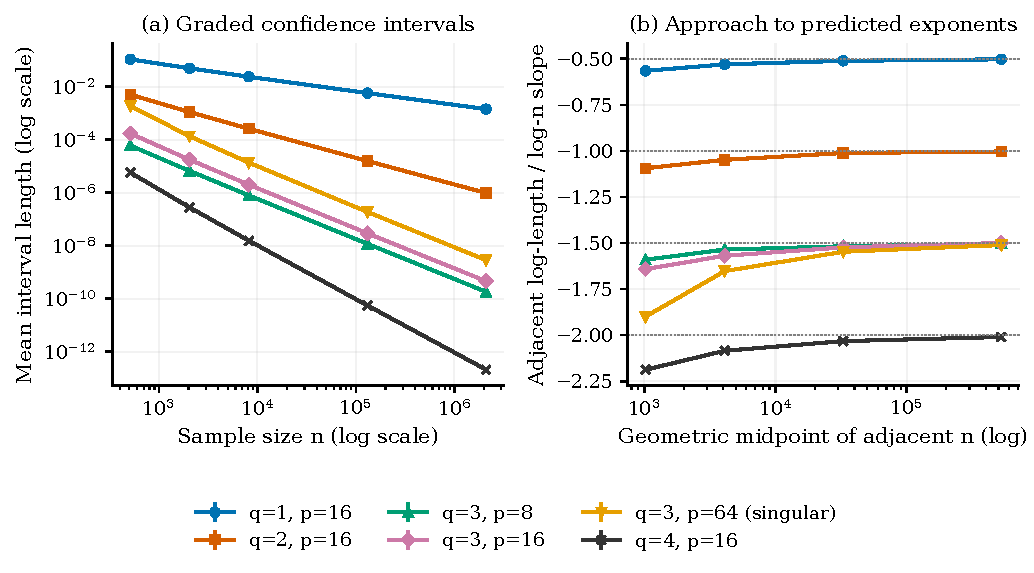
\includegraphics[width=\textwidth]{rates.pdf}
\caption{The graded interval exhibits contact orders one through four, with visible finite-dimension effects before the limiting regime. Each point uses 2,000 Gaussian datasets, $B_0=3E_{00\cdots0}$ and $A=E_{11\cdots1}$; mean-length bars are $\pm1.96$ Monte Carlo standard errors, often smaller than markers. The final two sample sizes are the disclosed addendum, and dotted slope guides mark $-q/2$.}\label{fig:rates}
\end{figure}

All graded intervals in the exactly specified contact experiments cover their targets. This demonstrates substantial conservatism. For example, at $n=2048$ in the four-way three-block setting, the mean graded length is $1.746\times10^{-5}$, compared with $1.741\times10^{-2}$ for the ambient scalar interval and $1.704\times10^{-8}$ for boundary-degree Wald. The last interval has empirical coverage 0.947 at the exact point but is not honest over its neighborhood. These numbers demonstrate a rate gain over ambient inference, not sharp constants or dominance over other valid minimum-distance constructions. In the $q=1$ slack setting, the graded ball is wider than the efficient scalar baseline.

\subsection{Rank activation and two prespecified functionals}
Use the path $B_{n,c}$ from Proposition~\ref{prop:wald}, with $c\in\{0,1,2,4,8\}$, $\lambda=3$ and $\sigma=0.2$. Its second central unfolding singular value is
\[
 \tau_2=\lambda|u_n|(1+u_n^2)
\]
for the values used here. It is zero at the boundary and is the smaller nonzero central singular value for $c>0$. The fixed loadings are
\[
 A_{\rm tan}=\frac{E_{0000}+0.35E_{0110}}{\sqrt{1+0.35^2}},
 \qquad A_{\rm normal}=E_{1111}.
\]
The first is substantially tangent aligned; the second is cubic normal at $c=0$ and nearly normal along the local path. Known-rank Wald uses an original-mode rank-one HOSVD when $c=0$ and the three-block HOSVD when $c>0$. Selected-rank Wald uses the former unless the second central singular value of OLS exceeds $\kappa\sigma\sqrt{2/n}$, with prespecified $\kappa=1,2,3$. These are diagnostic rank selectors, not asserted consistent selectors in a local-signal regime.

At $n=2048,c=2$, normal-loading coverage is 1.000 for graded inversion, 0.849 for known-rank Wald, 0.5525 for selected-rank Wald with $\kappa=2$, and 0.475 for boundary-degree Wald. The last value has Monte Carlo standard error about 0.0112. At $c=0$, its coverage is 0.9535. At $c=8$, it is 0.488, consistent with the approximately 0.4865 iterated limit in Proposition~\ref{prop:wald}. Thus knowledge of the actual rank does not remove functional degeneracy, and exact-boundary calibration does not provide uniform inference. For the tangent loading at $c=2$, corresponding known-rank and selected-$\kappa=2$ coverages are 0.9475 and 0.9255, showing a smaller but visible selection effect.

\subsection{Approximate structure and sensitivity}
For the four-way cubic loading, let $s_n=\tn^3/\lambda^2$. The allowance grid is
\[
 \eta\in\{0,s_n,100s_n,10000s_n,\tn^2/\lambda,\tn\}.
\] We evaluate both $B_0$ and the admissible departure $B_0+\eta A$, comparing exact-model and tube-aware graded intervals. At $n=2048$, $s_n=9.591\times10^{-9}$. A departure $\eta=\tn^2/\lambda=6.510\times10^{-6}$ reduces exact-model graded coverage to 0.847; tube-aware coverage is 1.000. At $\eta=10000s_n$, the exact-model interval has zero empirical coverage, while the tube-aware interval again covers in all replications and increases its mean length to $2.092\times10^{-4}$.

The honest interval's large finite-sample constants delay the visible transition relative to the asymptotic threshold $s_n$. It still covers all tested departures at $100s_n$ even though its exact-model guarantee does not apply there. This is consistent with a rate theorem whose constants are not sharp. Figure~\ref{fig:tube} shows both the cost of a known allowance at the exact point and the coverage consequence of ignoring a departure.

\begin{figure}[t]
\centering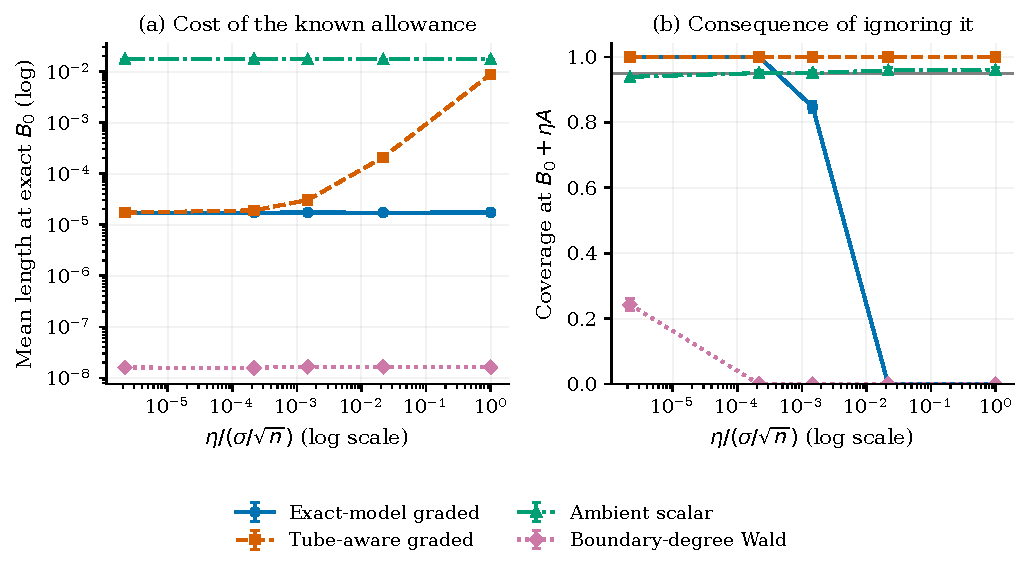
\includegraphics[width=\textwidth]{tube.pdf}
\caption{A known structural allowance increases honest length and protects against departures that invalidate exact-model inference. Four binary modes have caps $(1,2,1)$, $n=2048$, $\lambda=3$, $\sigma=0.2$, and $A=E_{1111}$. The left panel evaluates length at $B_0$ and the right coverage at $B_0+\eta A$, each with 2,000 replications; length bars are $\pm1.96$ Monte Carlo standard errors and coverage bars are Wilson 95\% Monte Carlo intervals.}\label{fig:tube}
\end{figure}

\subsection{Unknown noise, dense signals, and assumption diagnostics}
The study also varies $\lambda\in\{0.5,1,3\}$, rotates the signal and loading densely within modes, uses Gaussian design covariance $\Sigma_{ij}=0.5^{|i-j|}$, and evaluates the residual-$F$ procedure. The latter retains exact conditional coverage under Gaussian homoskedastic errors; a correlated full-rank design does not invalidate that statement. Dense rotations illustrate that coefficient sparsity is not needed.

Separate stress cases use standardized $t_5$ errors, heteroskedastic Gaussian errors, AR(1) errors with correlation 0.6, and Gaussian scale mixtures with 1\% or 5\% outlier probability and outlier standard deviation $5\sigma$. These cases are outside the exact noise theorem. For instance, at 5\% contamination the ambient interval using the uncontaminated $\sigma$ covers only 0.8045, while its residual-$t$ version covers 0.947 in this experiment. Conservative graded coverage at the tested boundary does not establish robustness to any of these departures. All diagnostic results, rather than only favorable settings, are included in the companion tables.
